\documentclass[10pt,pdftex]{report}
\usepackage[T1]{fontenc}
\usepackage[utf8]{inputenc}
\usepackage[magyar]{babel}
\usepackage{graphicx}
\usepackage{amsmath}
\usepackage{amssymb}
\usepackage{multirow}
\usepackage{booktabs}
\usepackage{indentfirst}
\usepackage[a4paper]{geometry}
\usepackage{url}
\usepackage{titling}
\usepackage{float}
\usepackage{adjustbox}
\usepackage{hyperref}
\usepackage{ dsfont }
\usepackage{xcolor}
\usepackage{amsmath}
    \definecolor{titlebg}{RGB}{128,128,128}

\usepackage{lmodern}
\usepackage{etoolbox}
\patchcmd{\thebibliography}{\chapter*}{\section*}{}{}

\renewcommand{\thesection}{\arabic{section}}


\title{Súrlódási együttható mérése}

%% EZ ALÁBBI KÉT MEZŐT ÉRTELEMSZERŰEN KI KELL TÖLTENI
\author{Bíró Gergő Tamás}
\date{2025. február 25.}


%% FEJLÉC LEÍRÓ, NEM KELL MÓDOSÍTANI
\renewcommand*{\maketitle}{\noindent\colorbox{titlebg}{%
\parbox{\dimexpr\linewidth-2\fboxsep}{\color{white}%
\parbox{\linewidth}{\fontsize{18}{24}\selectfont\sffamily\bfseries\thetitle}%
}}\vskip 1em%
\begin{tabular}{l}%
Mérést végezte: \theauthor \\%
Neptudnkód: R9SZLJ \\
Mérés dátuma: \thedate\\
Jegyzőkönyv végleges változata: \today %
\end{tabular}%
}
%%%%%%%%%%%%%%%%%%%%%

\begin{document}
\maketitle

%% ÉRDEMI MUNKA HELYE
\section*{Mérés célja}
A mérés során a motorokra erősített hengerek és a kapott üvegrúd közötti csúszási súrlódási együtthatót, ehhez az egyes motorok fordulatszámának 
feszültségfüggését is meg kell határoznunk, valamint a hengerekre helyezett rezgő mozgást végző rúd  periódusidejének a motorokba táplált feszültségtől való függését is 
szeretnénk meghatározni.
\section*{Mérési feladatok dokumentációja}
\subsection*{Mérőeszközök}
\begin{itemize}
    \item{Két elektromotor, rájuk erősített belül vályattal rendelkező műanyag hengerek.}
    \item{Mérőszalag}
    \item{Oszciloszkóp}
    \item{Tápegység}
\end{itemize}
\section*{Mérés leírása}
Első lépésként a motorokat kalibráljuk, olyan módon, hogy a motor tengelyére rögzített fekete korong fehér csíkjának fordulatszámát mérjük egy optikai reflexiós szenzor 
segítségével, aminek a jelét az oszciloszkóppal tudjuk leolvasni, ennek a frekvenciája meg fog egyezni a motor fordulatszámával. A motor fordulatszámát ilyen módon az 
$1,6-3,6V$ tartományon mérjük a kapott adatokra függvényt illesztünk, aminek segítségével meghatározzok a motor fordulatszámának feszültségtől való függését.
Ezután az első motorba a megadott $2.0V$-os, míg a másik motorba az azonos fordulatszámoz szükséges feszültséget táplálva mérjük a motorok feszültségváltozásának periódusidejét 
különböző motorok közötti távolsággal, ez az mért periódusidő meg fog egyezni a rúd rezgésének a periódusidejével. Végül a periódusiő fordulatszámfüggését az előzőhöz hasonló módon 
fogjuk mérni annyi eltéréssel, hogy ebben az esetben a motorok közötti távolságot tartjuk állandónak, és a motorok fordulatszámát változtatjuk.
\section*{Mérési adatok kiértékelése}
\subsection*{Elméleti előkészítés}
Megfigyelhetjük, hogy a $x(t)=x_0+A\mathrm{e}^{\beta t}\sin\left(\frac{2\pi}{T}t+\phi_0\right)$ függvénynek a maximumának helyébe az $A\mathrm{e}^{\beta t}$ nem fog beleszólni, 
valamint két szomszédos maximum helyének távolságába már $x_0$ és $\phi_0$ sem fognak. Innen már észrevehető, hogy a szomszédos maximumhelyek $t=T$ távolságra vannak egymástól.
\newline
A rúd sebességének a függvényét a kitérésfüggvény deriválásával kaphatjuk meg, amelyre a következő adódik:
\begin{equation}
    v(t)=A\mathrm{e}^{\beta t}\left(\beta\sin\left(\frac{2\pi}{T}t+\phi_0\right)+\frac{2\pi}{T}\cos\left(\frac{2\pi}{T}t+\phi_0\right)\right) \label{eq:1}
\end{equation}
\eqref{eq:1}-ből láthatjuk, hogy amennyiben $\beta>0$ a sebességének nem lesz maximuma, $\beta\leq 0$ esetben pedig a lehető legnagyobb sebesség $t=0$-ban lesz 
kiszen ekkor még nem kezdett el csökkenni a rezgés amplitúdója. \eqref{eq:1} értéke 0-ban pedig láthatóan akkor a legnagyobb, ha $\cos\left(\frac{2\pi}{T}t+\phi_0\right)$ 
értéke $\pm 1$, ami abban az esetben van ha $\phi_0=n\pi, n\in\mathds{Z}$. Ekkor $v_{max}=A\frac{2\pi}{T}$ adódik.\\A rúd akkor fog mindig csúszni a hengereken, ha 
$v_k>v_{rúd}$ minden időpillanatban, ahol $v_k$ a hengerek kerületi sebessége abban a sugárban, ahol a rúddal érintkeznek, amiből következik, hogy $v_k>v_{max}$ összefüggésnek is igaznak kell lennie. 
Ezt átírva a következő egyenletre jutunk:
\begin{equation}
    2\pi fr>A\frac{2\pi}{T} \label{eq:2}
\end{equation}
Amegadott $A=25cm$, $r=2cm$, $T=2s$ paramétereket \eqref{eq:2}-be helyettesítve pedig a fordulatszámra $f>6.25Hz$ adódik.
\subsection*{Motorok kalibrálása}
A motorok kalibrálása során az adott feszültségekez tartozó fordulatszámot az oszciloszkóp automatikusan mérte, ám a kapott értékek nem voltak időben állandóak, igy 
feszültségenként ötször olvastuk le az adatokat, ezeknek az átlagát tekisük a fordulatszám értékének, míg a a hibájuk a megfelelő feszültséghez tartozó adatoknak a szórása lesz.\\
\begin{table}[H]
    \begin{tabular}{|r|r|r|r|r|r|}
        \hline
        Feszültség$(V)$ & 1. mérés$(Hz)$ & 2. mérés$(Hz)$ & 3. mérés$(Hz)$ & 4. mérés$(Hz)$ & 5. mérés$(Hz)$ \\
        \hline
        1.6 & 11.996 & 11.959 & 11.950 & 11.653 & 11.632 \\
        \hline
        1.8 & 13.927 & 13.908 & 13.665 & 13.500 & 13.429 \\
        \hline
        2.0 & 16.191 & 16.000 & 16.127 & 15.935 & 15.791 \\
        \hline
        2.2 & 17.976 & 17.871 & 18.149 & 17.875 & 18.057 \\
        \hline
        2.4 & 20.374 & 20.220 & 20.329 & 20.145 & 20.293 \\
        \hline
        2.6 & 22.510 & 22.314 & 22.969 & 22.411 & 22.669 \\
        \hline
        2.8 & 24.487 & 24.605 & 24.398 & 24.759 & 25.012 \\
        \hline
        3.0 & 26.695 & 26.729 & 27.075 & 26.873 & 27.165 \\
        \hline
        3.2 & 29.059 & 29.078 & 28.985 & 28.865 & 28.920 \\
        \hline
        3.4 & 31.353 & 31.593 & 31.349 & 31.183 & 31.472 \\
        \hline
    \end{tabular}
    \caption{1. motor fordulatszáma különböző feszültségek mellett.}
\end{table}
\begin{table}[H]
    \begin{tabular}{|r|r|r|}
        \hline
        Feszültség$(V)$ & Átlag fordulatszám$(Hz)$ & Fordulatszám szórása$(Hz)$ \\
        \hline
        1.6 & 11.838 & 0.02576 \\
        \hline
        1.8 & 13.686 & 0.04169 \\
        \hline
        2.0 & 16.009 & 0.02003 \\
        \hline
        2.2 & 17.986 & 0.01145 \\
        \hline
        2.4 & 20.272 & 0.00659 \\
        \hline
        2.6 & 22.575 & 0.05266 \\
        \hline
        2.8 & 24.652 & 0.04700 \\
        \hline
        3.0 & 26.907 & 0.03451 \\
        \hline
        3.2 & 28.981 & 0.00654 \\
        \hline
        3.4 & 31.390 & 0.01877 \\
        \hline
    \end{tabular}
    \caption{1. motor fordulatszáma, és annak hibája a betáplált feszültség függvényében.}
\end{table}
\begin{table}[H]
    \begin{tabular}{|r|r|r|r|r|r|}
        \hline
        Feszültség$(V)$ & 1. mérés$(Hz)$ & 2. mérés$(Hz)$ & 3. mérés$(Hz)$ & 4. mérés$(Hz)$ & 5. mérés$(Hz)$ \\
        \hline
        1.6 & 13.373 & 13.730 & 13.784 & 13.896 & 13.762 \\
        \hline
        1.8 & 16.020 & 16.171 & 16.199 & 16.096 & 15.838 \\
        \hline
        2.0 & 17.659 & 17.983 & 17.899 & 17.980 & 17.910 \\
        \hline
        2.2 & 20.266 & 20.224 & 20.210 & 19.887 & 19.893 \\
        \hline
        2.4 & 22.255 & 22.044 & 22.068 & 21.997 & 21.771 \\
        \hline
        2.6 & 24.717 & 24.529 & 24.448 & 24.470 & 24.519 \\
        \hline
        2.8 & 26.543 & 26.303 & 26.308 & 26.597 & 26.431 \\
        \hline
        3.0 & 28.617 & 28.702 & 28.519 & 28.666 & 28.704 \\
        \hline
        3.2 & 31.082 & 31.075 & 31.340 & 31.328 & 31.104 \\
        \hline
        3.4 & 33.308 & 33.440 & 33.420 & 33.586 & 33.489 \\
        \hline
    \end{tabular}
    \caption{2. motor fordulatszáma különböző feszültségek mellett.}
\end{table}
\begin{table}[H]
    \begin{tabular}{|r|r|r|}
        \hline
        Feszültség$(V)$ & Átlag fordulatszám$(Hz)$ & Fordulatszám szórása$(Hz)$ \\
        \hline
        1.6 & 13.709 & 0.03135 \\
        \hline
        1.8 & 16.065 & 0.01674 \\
        \hline
        2.0 & 17.886 & 0.01410 \\
        \hline
        2.2 & 20.096 & 0.02863 \\
        \hline
        2.4 & 22.027 & 0.02408 \\
        \hline
        2.6 & 24.537 & 0.00904 \\
        \hline
        2.8 & 26.436 & 0.01429 \\
        \hline
        3.0 & 28.642 & 0.00475 \\
        \hline
        3.2 & 31.186 & 0.01475 \\
        \hline
        3.4 & 33.449 & 0.00823 \\
        \hline
    \end{tabular}
    \caption{2. motor fordulatszáma, és annak hibája a betáplált feszültség függvényében.}
\end{table}
A fenti táblázatokban kapott adatokra motoronként $ax+b$, $ax^2+bx+c$ és $ax+b\sqrt{x}+c$ függvényeket illesztünk, a lehetőségek közül az adatokkal leginkább 
egyező illesztéből származó összefüggést fogjuk használni a további mérések során. Az illesztésekből a következő összefüggéseket kaptuk:\\
\begin{table}[H]
    %\begin{adjustbox}{width=1\textwidth}
        \begin{tabular}{|r|r|r|}
            \hline
            Motor száma & Illesztésből kapott összefüggés\footnotemark\footnotetext{AZ alábbiakban U a motorba tápált feszültséget, 
            f pedig a motor fordulatszámát fogja jelölni.} & Illesztés paramétereinek hibája\footnotemark \\
            \hline
            1. & $f=10.908U-5.904$ & 0.057, 0.155 \\
            \hline
            1. & $f=0.238U^2+9.635U-4.258$ & 0.117, 0.633, 0.826 \\
            \hline
            1. & $f=13.09119058U-7.08460039\sqrt{U}-0.20552651$ & 1.081, 3.504, 2.822 \\
            \hline
            2. & $f=10.906U-3.924$ & 0.158, 0.459 \\
            \hline
            2. & $f=0.612U^2+7.690U+0.153$ & 0.212, 1.124, 1.456 \\
            \hline
            2. & $f=16.905U-19.249\sqrt{U}+11.367$ & 2.322, 7.440, 5.921 \\
            \hline
        \end{tabular}
    %\end{adjustbox}
    \caption{Az egyes motorok esetbén az illesztésből származó összefüggés.}
\end{table}
\footnotetext{A felsorolt hibák a hozzájuk tartozó paraméterek sorrendjében vannak elhelyezve a cellában.}
\begin{figure}
    \centering
    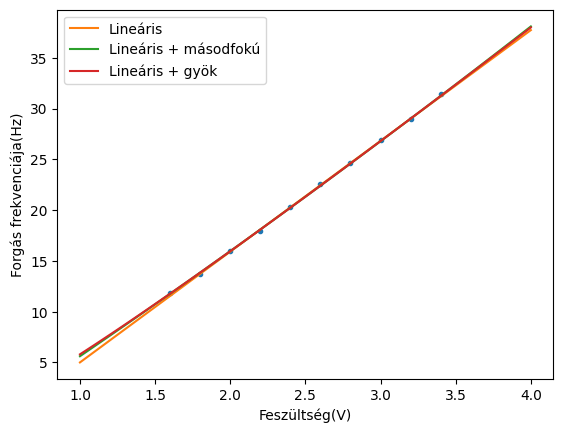
\includegraphics[scale=0.5]{Motor_1.png}
    \caption{Az első motoron mért adatok, a rá illisztett függvények.}
\end{figure}
\begin{figure}[H]
    \centering
    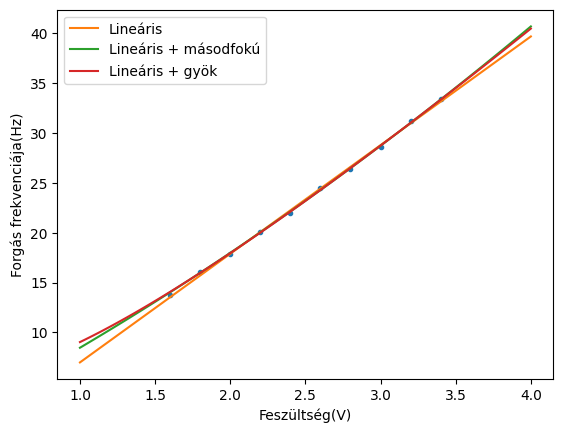
\includegraphics[scale=0.5]{Motor_2.png}
    \caption{A második motoron mért adatok, a rá illisztett függvények.}
\end{figure}
A fenti képeken is megfigyelhető, hogy mindhárom illesztés közel azonosan illeszkedik a mért adatpontokra, azonban a másodfokú vagy gyökös tagot tartalmazó 
függvények hibája jelentősen nagyobb a lineáris függvényekénél, így érdemes a lineáris összefüggést használni a továbbiakban.\\
A kalibrációs táblázat, a következő mérésekben használt feszültségekhez, melyeken a fordulatszámok megegyeznek:\\
\begin{table}[H]
    \begin{tabular}{|r|r|}
        \hline
        1. Motorba táplált feszültség$(V)$ & 2. Motorba táplált feszültség$(V)$\\
        \hline
        1.60 & 1.42 \\
        \hline
        1.70 & 1.52 \\
        \hline
        1.80 & 1.62 \\
        \hline
        1.90 & 1.72 \\
        \hline
        2.00 & 1.82 \\
        \hline
        2.10 & 1.92 \\
        \hline
        2.20 & 2.02 \\
        \hline
        2.30 & 2.12 \\
        \hline
        2.40 & 2.22 \\
        \hline
        2.50 & 2.32 \\
        \hline
    \end{tabular}
    \caption{A mérések során használt motorokba tápűlált feszültségek páronként \footnotemark.}
\end{table}
\footnotetext{Az értékek azért vannak 2 tizedesjegyre kerekítve, mivel ilyen pontossággal lehet változtatni a betáplált feszültséget.}
A kapott adatokra ha ismént lineáris, valamint lineáris és gyökös vagy másodfokú tagaot tartalmazó függvényt illesztve azt figyelhetjük meg, hogy a lineáris, és a konstans tag 
mellett a másodfokú. és a gyököt tartalmazó tagok együrtthatója elhanyagolhatóak, így ismét érdemes a lineáris függvényt használni, melynek egyenlete: $U_2=1.003U_1-0.189$, 
amiben a lineáris tag hibája $2.606\cdot 10^{-17}$, a konstans tagé pedig $5.732\cdot 10^{-17}$.
\begin{figure}[H]
    \centering
    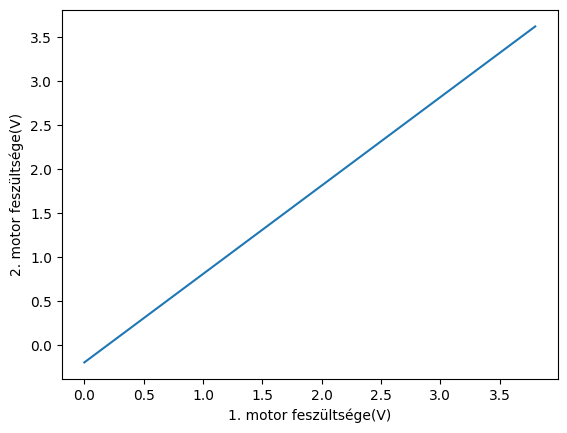
\includegraphics[scale=0.5]{Kalibracio.png}
    \caption{Motorok feszültsége a máik feszültségéhez képest, abban az esetben, amikor a fordulatszámuk megegyezik.}
\end{figure}
\subsection*{Elméleti modell a rúd periódusidejének súrlódástó való függéséhez}
Legyen a két alátámasztási ponton fellépő erő nagysága $F_1$ és $F_2$ ezekről tudjuk,\\ hogy $F_1+f_2=mg$, ahol $m$ a rúd tömege, $g$ pedig a nehézségi gyorsulás. 
Ha a rúd kitérése a középponthoz képest $x$, akkor a rúd közepére a forgatónyomatékogy egyenlőségét felírva a következő egyenletet kapjuk:
\begin{equation*}
    F_1\left(\frac{\ell}{2}+x\right)=F_2\left(\frac{\ell}{2}-x\right)
\end{equation*}
Amiben $\ell$ a rúd hossza. Az egyenletrendszer megoldása a következő lesz:
\begin{eqnarray*}
    F_1=\frac{\frac{\ell}{2}-x}{l}\\
    F_2=\frac{\frac{\ell}{2}+x}{l}
\end{eqnarray*}
Mivel a két henger forgásának iránya ellentétes a vízszintes irábnyú erők eredője a következő lesz:
\begin{equation*}
    F=m\ddot{x}=\mu\left(F_1-F_2\right)=-\mu\sqrt{2}mg\frac{2x}{l}
\end{equation*}
Ahol $\mu$ a súrlódási együttható. A fenti képletben a $\sqrt{2}$-es szorzó abból adódik, hogy a rúd két egymással $90^{\circ}$-ot bezáró kúppal van alátámaszva mindkét 
alátámasztási ponton. A fent látható differenciálegyenletből pedig a periódusiőre a következő összefüggést kapjuk:
\begin{equation*}
    T=\frac{2\pi}{\omega_0}=\frac{2\pi}{\sqrt{\frac{D^*}{m}}}=2\pi\sqrt{\frac{l}{\mu 2\sqrt{2}g}}
\end{equation*}
Akol $T$ a periódusiő, $\omega_0$ pedig a rezgés körfrekvenciája.
\subsection*{Súrlódási együttható meghatározása}
A súrlódási együttható meghatározása során az 1. motorba táplált feszültség $U_1=2.00V$, a 2. motorba táplált feszültség pedig $U_2=1.82V$ volt.
A kalibráció során ezen a feszültségen mért fordulatszámok $16Hz$ körül voltak, melyek nagyobbak az elméleti előkészület alatt kiszámolt minimális értéknél. \\
\begin{table}[H]
    \begin{tabular}{|r|r|r|r|}
        \hline
        Hengerek tengelye közti távolság$(m)$ & Mért idő$(s)$ & Mért idő hibája$(s)$ & Mért periódusok száma \\
        \hline
        0.526 & 7.314 & 0.222 & 4 \\
        \hline
        0.506 & 5.289 & 0.180 & 3 \\
        \hline
        0.460 & 6.943 & 0.191 & 4 \\
        \hline
        0.569 & 7.557 & 0.232 & 4 \\
        \hline
        0.620 & 7.901 & 0.254 & 4 \\
        \hline
        0.712 & 6.179 & 0.191 & 3 \\
        \hline
        0.316 & 5.787 & 0.138 & 4 \\
        \hline
        0.533 & 7.536 & 0.127 & 4 \\
        \hline
        0.594 & 5.872 & 0.223 & 3 \\
        \hline
        0.628 & 5.978 & 0.212 & 3 \\
        \hline
    \end{tabular}
    \caption{Súrlódási együttható meghatározásához mért adatok.}
\end{table}
\begin{table}[H]
    \begin{tabular}{|r|r|r|}
        \hline
        Hengerek tengelye közti távolság$(m)$ & Mért idő$(s)$ & Mért idő hibája$(s)$ \\
        \hline
        0.526 & 1.829 & 0.056 \\
        \hline
        0.506 & 1.763 & 0.060 \\
        \hline
        0.460 & 1.736 & 0.048 \\
        \hline
        0.569 & 1.890 & 0.058 \\
        \hline
        0.620 & 1.975 & 0.064 \\
        \hline
        0.712 & 2.060 & 0.064 \\
        \hline
        0.316 & 1.447 & 0.035 \\
        \hline
        0.533 & 1.884 & 0.032 \\
        \hline
        0.594 & 1.957 & 0.074 \\
        \hline
        0.628 & 1.993 & 0.071 \\
        \hline
    \end{tabular}
    \caption{Súrlódási együttható meghatározásához mért adatok egy periódusra normálva.}
\end{table}
A fenti táblázatban az összes hosszúsághoz tartozik egy $\Delta l=\pm0.0005m$-es hiba, amely a mérőszalag ponosságából adódik. A mért idő hibája az oszciloszkómon 
megfigyelhető jel maximumának pontatlan meghatározásából származik, mivel amikor a rúd jobban terhelte az adott motort a szinuszgörbe csúcsa eltorzult, ez az alábbi képeken 
is megfigyelhető:\\
\begin{figure}[H]
    \centering
    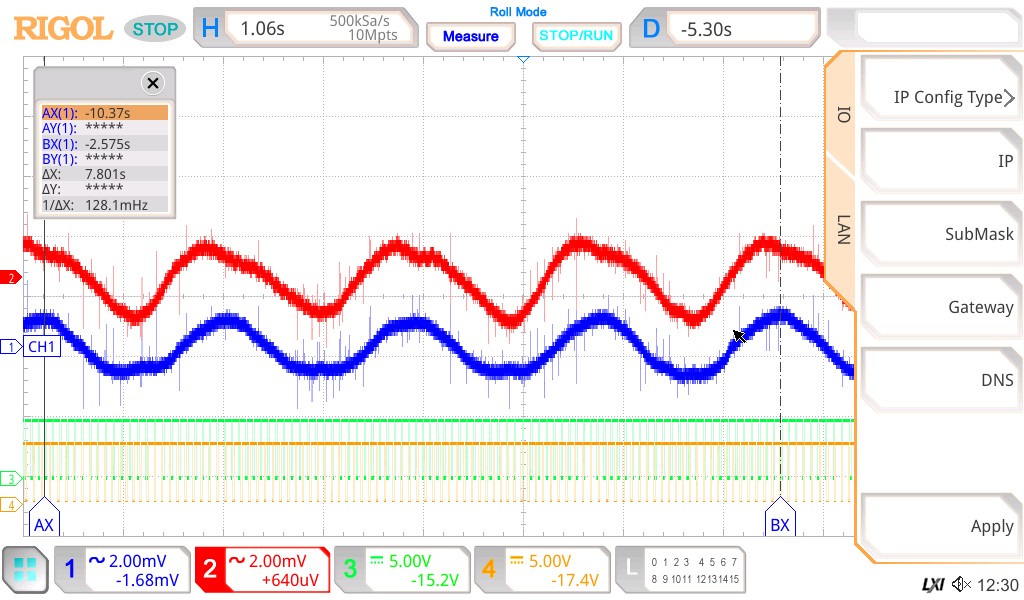
\includegraphics[scale=0.5]{Meres_5.png}
\end{figure}
\begin{figure}[H]
    \centering
    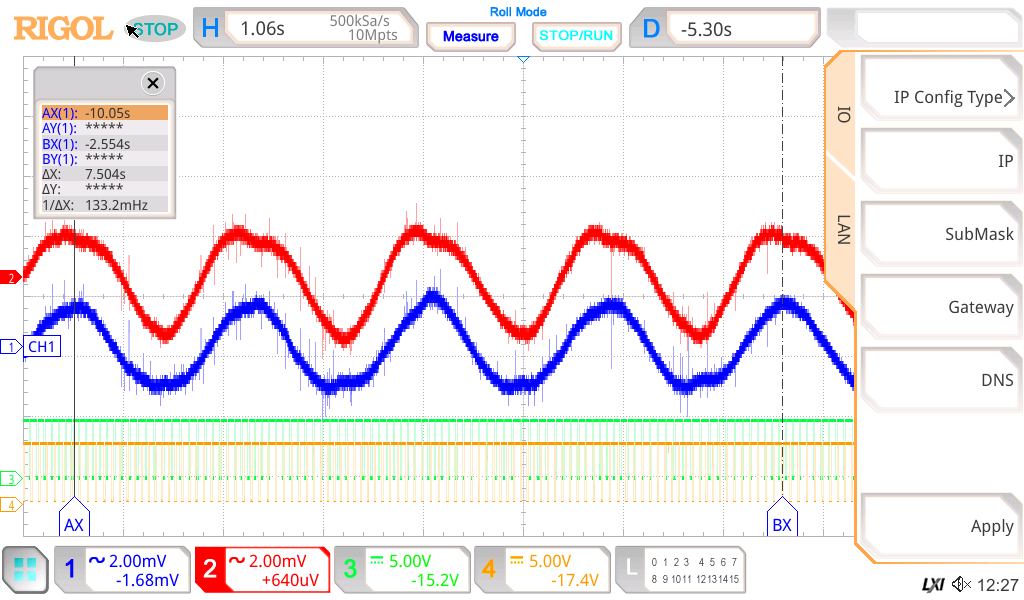
\includegraphics[scale=0.5]{Meres_4.png}
\end{figure}
Az oszciloszkópokon látható jelben még megfigyelhető szinusztól való eltérések magyarázata lehet a rúd rezgése, amely azért probléma, mert íny nem ugyanakkora minden 
időpillanatban a nyomóerő, mintha a rúd nem rezegne. Ezen felül még az is beleszólhatott a a jel torzulásába, hogy kisebb feszültségek esetében a motorok fordulatszáma 
jelentősen megváltozhatott a terheléstől.\\

A kapott adatokra $K_0\ell^{\alpha}$ függvényt illesztve $K_0$-értékére $2.45987676\pm0.03842954$ adódik, $\alpha$-ra pedig $0.45409613\pm0.02231953$.
\begin{figure}[H]
    \centering
    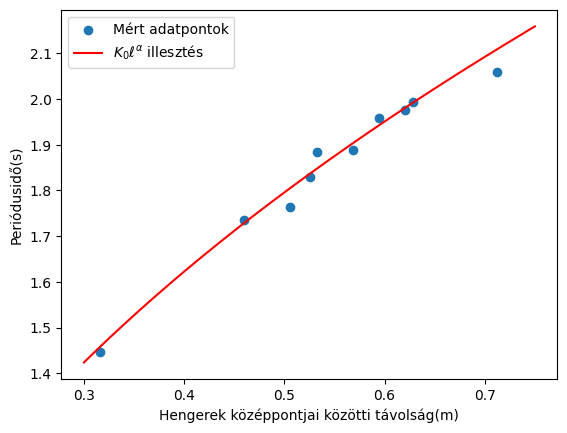
\includegraphics[scale=0.5]{Illesztes_alpha.png}
    \caption{$K_0\ell^{\alpha}$ alakú illesztett függvény.}
\end{figure}
A kapott $\alpha$ érték közel van az elméleti modell $\alpha=0.5$ értékével, az eltérés magyarázható a rúd rezgésével, és a két motor fordulatszámingadozásával.\\
Az elméleti modellben megadott összefüggés az alátámasztási pontok közötti távolság, és a periódusidő között:
\begin{equation}
    T=2\pi\sqrt{\frac{\ell}{\mu\sqrt{8}g}} \label{eq:3}
\end{equation}
Ami ben nevezzük el $\frac{4\pi^2}{\mu\sqrt{8}g}$ $K$-nak. Ezzel a helyettesítéssel \eqref{eq:3} új formája:
\begin{equation}
    T=K^{0.5}\ell^{0.5} \label{eq:4}
\end{equation}
\eqref{eq:4} az $\alpha=0.5$ esetben adódik, így általánosan a következő adódik:
\begin{equation}
    T=K^{\alpha}\ell^{\alpha}=\left(\frac{4\pi^2}{\mu\sqrt{8}g}\right)^{\alpha}\ell^{\alpha} \label{eq:5}
\end{equation}
Ahol $K^{\alpha}=K_0$.
\eqref{eq:5}-ből $\mu$-t  kifejezve a súrlódási együttható értékére a következő összefüggés adódik:
\begin{equation}
    \mu=\frac{\left(4\pi^2\right)^{1/\alpha}}{\sqrt{8}g}\frac{\ell}{T^{1/\alpha}}=\frac{\left(4\pi^2\right)^{1/\alpha}}{\sqrt{8}g}\frac{1}{K_0^{1/\alpha}} \label{eq:6}
\end{equation}
Ahol 
\eqref{eq:6}-ból pedig a súrlódási együttható értékére $\mu=0.2842\pm5.4479$ adódik, ahol $\mu$ hibáját a következő képlet adja meg:
\begin{equation}
    \Delta\mu=\left|\frac{\partial \mu}{\partial \alpha}\right|\Delta\alpha+\left|\frac{\partial \mu}{\partial K_0}\right|\Delta K_0 \\ \label{eq:7}
\end{equation}
Annak az oka, hogy a hiba egy nagyságrenddel nagyobb, mint a kapott értéké az, hogy jelen esetben a használt hibaterjedési modell nem megfelelő az exponeciális függvény 
pontos hibájának megadására, amennyiben $\alpha$ hibáját figyelmen kívül hagynánk még akkor is jelentős $\Delta\mu=0.5598$ hibát kapnánk.\\
Az $\alpha=0.5$ esetben illesztett függvényre $K_0=2.53555221\pm0.01470517$ adódik, amiből a súrlódási együtthatóra $\mu=0.2213\pm0.1013$-et kapunk. Ez a másik eseből származó 
értékkel összehasonlítható mértékű, ekkora különbség reálisan adódhat a motorok hibáiból, és a rúd rezgése miatti nem állandó nyomóerőből. A két érték hibahatáron belül van egymáshoz 
képest, azonban mindkét esetben a hibaterjedés pontatlan modellje miatt a súrlódási együttható, és annak a hibája azonos nagyságrendűek.
\begin{figure}[H]
    \centering
    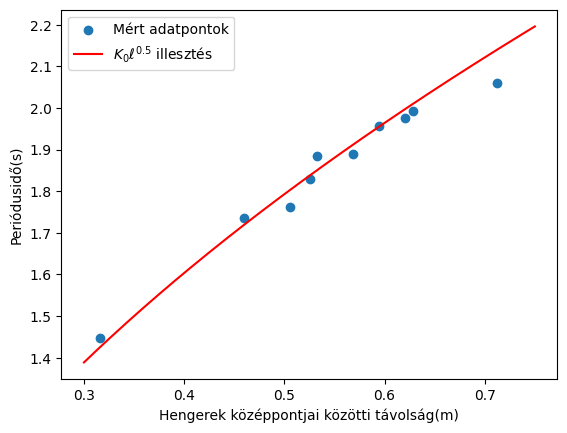
\includegraphics[scale=0.5]{Illesztes_05.png}
    \caption{$K_0\ell^{0.5}$ alakú illesztett függvény.}
\end{figure}
\subsection*{A periódusidő fordulatszám függésének vizsgálata}
Ez alatt a mérés alatt a két motor tengelye közötti távolság $\ell=0.587\pm0.0005m$ volt, a mérés során a következő adatokat kaptudk:\\
\begin{table}[H]
    \begin{tabular}{|r|r|r|r|r|}
        \hline
        1. motor feszültsége$(V)$ & 2.motor feszültsége$(V)$ & Mért idő$(s)$ & Mért idő hibája$(s)$ & Mért periódusok száma \\
        \hline
        1.6 & 1.42 & 5.967 & 0.286 & 3 \\
        \hline
        1.7 & 1.52 & 7.685 & 0.254 & 4 \\
        \hline
        1.8 & 1.62 & 9.667 & 0.191 & 5 \\
        \hline
        1.9 & 1.72 & 9.688 & 0.192 & 5 \\
        \hline
        2.0 & 1.82 & 9.561 & 0.180 & 5 \\
        \hline
        2.1 & 1.92 & 9.540 & 0.159 & 5 \\
        \hline
        2.2 & 2.02 & 9.582 & 0.191 & 5 \\
        \hline
        2.3 & 2.12 & 9.571 & 0.212 & 5 \\
        \hline
        2.4 & 2.22 & 9.656 & 0.180 & 5 \\
        \hline
        2.5 & 2.32 & 7.748 & 0.170 & 5 \\
        \hline
    \end{tabular}
    \caption{Mért periódusidők több fordulatszámhoz.}
\end{table}
\begin{table}[H]
    \begin{tabular}{|r|r|r|r|}
        \hline
        1. motor feszültsége$(V)$ & 2.motor feszültsége$(V)$ & Mért idő$(s)$ & Mért idő hibája$(s)$ \\
        \hline
        1.60 & 1.42 & 1.989 & 0.095 \\
        \hline
        1.70 & 1.52 & 1.921 & 0.064 \\
        \hline
        1.80 & 1.62 & 1.933 & 0.038 \\
        \hline
        1.90 & 1.72 & 1.938 & 0.038 \\
        \hline
        2.00 & 1.82 & 1.912 & 0.036 \\
        \hline
        2.10 & 1.92 & 1.908 & 0.032 \\
        \hline
        2.20 & 2.02 & 1.916 & 0.038 \\
        \hline
        2.30 & 2.12 & 1.914 & 0.042 \\
        \hline
        2.40 & 2.22 & 1.931 & 0.036 \\
        \hline
        2.50 & 2.32 & 1.550 & 0.034 \\
        \hline
    \end{tabular}
    \caption{Mért periódusidők több fordulatszámhoz, egy periódusra normálva.}
\end{table}
A kapott periódusidőket az 1. motor feszültségének függvényében a következő ábrát kapjuk:
\begin{figure}[H]
    \centering
    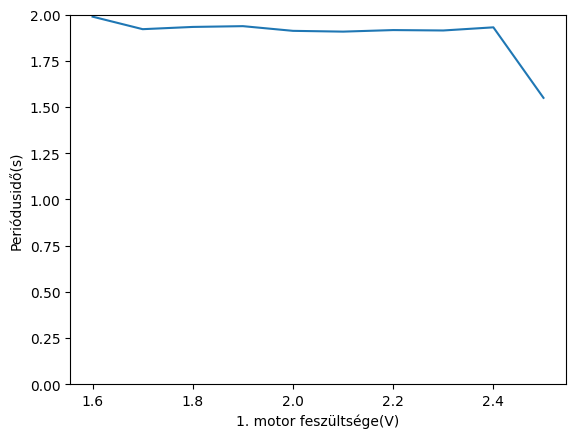
\includegraphics[scale=0.5]{Periodusidok.png}
\end{figure}
Ezen megfigyelhetjük, hogy a periódusidő tényleg egy közel konstans értéket vesz fel minden feszültség mellett az utolsó adatpontot leszámítva, ami olyan jelentősen eltér 
a többi adatponttól, amiből fel lehet tételezni, hogy az eltérést egy hibás mérés okozta. A kritikus fordulatszám alá egyszer sem ment a fordulatszám a mért intervallumon, 
így nem látszik az az alatt lévő fordulatszámok esetén a periódusidő fordulatszámfüggése, ám ott már nem lesz független a két mennyiség, hoszen nem fog folyamatosan hatni a súrlódási 
erő a rúdra, mivel az nem fog minden időpillanatban csúszni.
\section*{Összegzés}
A mérés során kapott súrlódási együtthatók reális nagyságúnak adódtak, a vártaknak megfelelően 0 és 1 közé esett mindkét számítási módszerrel az értéke 
azonban a hibája jelentős, amely első sorban a választott hibaterjedési modll pontatlanságából származik. A periódusidőnek a motorok fordulatszámától vasó 
függetlenségét is sikerült igazolni, amennyiben az egyetlen a többitől jelentősen eltérő adatpot a várttól való eltérését egy mérési hiba okozta.
%% IRODALOMJEGYZÉK
%\begin{thebibliography}{9}

%\bibitem{lamport94}
%  Leslie Lamport,
%  \textit{\LaTeX: a document preparation system},
%  Addison Wesley, Massachusetts,
%  2nd edition,
%  1994.
%  \url{https://bla.com}

%\end{thebibliography}

\end{document}
